\documentclass[conference]{IEEEtran}
\usepackage[T1]{fontenc}
\usepackage[utf8]{inputenc}
\usepackage{cite}
\usepackage{url}
\usepackage{hyperref}
\usepackage{graphicx}
\usepackage{booktabs}
\usepackage{array}
\usepackage{multirow}
\usepackage{amsmath}
\usepackage{amssymb}
\usepackage{algorithm}
\usepackage{algorithmic}
\usepackage{float}
\usepackage{xcolor}
\usepackage{enumitem}
\usepackage{balance}
\usepackage{tikz}
\usetikzlibrary{arrows.meta, positioning, shapes.geometric, shapes.misc, fit, calc}

\hypersetup{
    colorlinks=true,
    linkcolor=blue,
    citecolor=blue,
    urlcolor=blue,
    pdftitle={MedAI: A Full-Stack AI-Assisted Healthcare Platform with MedMNIST-Based Medical Image Diagnosis},
    pdfauthor={Generated Draft}
}

\title{MedAI: A Full-Stack AI-Assisted Healthcare Platform with MedMNIST-Based Medical Image Diagnosis}

\author{
\IEEEauthorblockN{Gorrepati Varshith$^{1}$, 
Vuriti Tirumala Srinivas$^{2}$, 
Andra Hema Swaroop$^{3}$,\\
Cheruku Ganesh$^{4}$, 
Prabhujit Mohapatra$^{5}$*}
\IEEEauthorblockA{Department of Computer Science, SRM University, Andhra Pradesh, India\\
$^{1}$varshithgorrepati3366@gmail.com,
$^{2}$tirumalasrinivas\_vuriti@srmap.edu.in,
$^{3}$hemaswaroop\_andra@srmap.edu.in,\\
$^{4}$ganesh\_cheruku@srmap.edu.in,
$^{5}$prabhujit.m@srmap.edu.in\\
*Corresponding author}
}


\begin{document}
\maketitle

\begin{abstract}
MedAI is a full-stack healthcare web platform that combines conversational AI, image-based medical assessment, patient self-management, clinician workflows, and administrative oversight in one application. The system pairs a FastAPI backend with a React and Vite frontend, MongoDB persistence, Redis-backed runtime support, role-aware access control, and a modular AI layer for chat, retrieval-augmented generation, document extraction, and image understanding.

The current branch centers the medical image diagnosis pipeline on MedMNIST-compatible inference with EfficientNet-B0 classifiers. Rather than treating diagnosis as generic text reasoning, the platform uses uploaded medical images as the primary signal and converts the prediction into downstream care guidance such as specialty referral, suggested tests, treatment context, and explicit safety disclaimers. This paper describes the architecture, service decomposition, modality normalization, and operational design choices that make the system practical to extend and deploy.
\end{abstract}

\begin{IEEEkeywords}
Healthcare AI, medical image diagnosis, MedMNIST, EfficientNet-B0, FastAPI, React, retrieval-augmented generation, multi-modal healthcare systems, clinical decision support, web applications.
\end{IEEEkeywords}

\section{Introduction}
Healthcare software has been moving steadily toward integrated digital ecosystems in which patients, clinicians, and administrators operate within a shared platform rather than across disconnected tools. This trend is driven by several practical pressures. Patients want immediate answers, guided next steps, and convenient access to everyday healthcare workflows such as medication reminders, consultations, and test booking. Clinicians need concise triage information, structured summaries, and access to patient context without navigating fragmented systems. Administrators require observability over users, roles, analytics, and operational settings. Meanwhile, AI systems are increasingly expected to support more than generic text chat; they must operate across images, documents, and clinical knowledge sources while preserving safe use boundaries. MedAI is designed in response to these requirements.

The platform studied in this manuscript is a healthcare-oriented full-stack application that combines a broad set of functional modules. The user-facing side is implemented in React and Vite and includes routes for patient chat, health tracking, medicine reminders, pharmacy browsing, lab tests, prescriptions, consultations, profile management, and general support. Administrative and doctor-facing routes support dashboards, patient lists, appointment handling, prescriptions, settings, roles, analytics, and onboarding workflows. The backend is implemented in FastAPI and exposes structured APIs for authentication, chat, health logs, medicine support, pharmacy ordering, diagnosis, and auxiliary analytics. This architecture allows the system to operate as a single product while keeping each concern separated in code.

The current branch introduces a particularly important change in the diagnosis subsystem. In many healthcare chat applications, image input is treated as a generic prompt augmentation step, where the model is asked to infer meaning from a photo or a textual description. That approach is too loose for a meaningful clinical classification task. MedAI instead treats image diagnosis as a first-class pipeline with its own model loading, modality normalization, and confidence reporting logic. The implementation uses EfficientNet-B0 classifiers trained on supported MedMNIST 2D subsets and can map multiple image domains into corresponding medical categories. The pipeline does not merely return a label. It transforms the output into a structured result that includes disease prediction, confidence, top predictions, doctor specialty mapping, treatment context, suggested tests, and an explanatory response generated by an AI service with optional retrieval augmentation.

This design follows a pattern seen in recent medical imaging systems that pair task-specific models with clinical context, safety framing, and human-readable guidance rather than exposing raw predictions alone \cite{esteva,chexnet,topol,medmnistv2}.

The rationale for this design is straightforward. In practical healthcare applications, users rarely need a single isolated prediction. They need an answer that connects evidence to action. A skin lesion image, for example, is most useful when the system can identify the likely condition, indicate whether the confidence is above threshold, suggest the type of specialist to consult, and present a short explanation of why the model reached that conclusion. The same pattern applies to pathology slides, chest radiographs, retinal images, or other MedMNIST modalities. By structuring the response around clinical follow-up rather than standalone classification, MedAI moves closer to a useful decision-support system.

Another motivation is architectural consistency. The backend already includes services for AI chat, document extraction, health analytics, reminders, and RAG. Rather than building a separate image analysis stack that is disconnected from the rest of the product, the diagnosis subsystem is integrated into the same service ecosystem. This means the application can apply common patterns such as error handling, logging, authentication, and route orchestration across different features. The design also makes it easier to extend the product: new modalities can be added by registering weight files and metadata, while existing routes continue to function.

This paper provides a detailed explanation of the implementation and organization of the system. Although the codebase is application-oriented rather than research-only, the combination of web engineering and medical AI raises interesting system design questions. How should a platform select and normalize medical image modalities? How can an AI service safely produce explanations without pretending to be a clinician? How can a frontend remain responsive when much of the application is role-based and feature-dense? How can a backend support both chat and image inference without conflating the two? We address these questions by analyzing the concrete structure of the project.

The main contributions are as follows:

\begin{itemize}[leftmargin=*,itemsep=2pt,topsep=4pt]
    \item A full-stack healthcare platform that unifies patient, doctor, and administrator workflows in a single monorepo.
    \item A MedMNIST-based medical image diagnosis pipeline with modality normalization, EfficientNet-B0 inference, and structured response generation.
    \item A clear separation between general chat, document extraction, and clinical image inference to reduce unsafe task conflation.
    \item An application-level response design that connects prediction output to specialty routing, test suggestions, and next-step guidance.
\end{itemize}

The remainder of this manuscript is organized as follows. Section II summarizes the system requirements and design goals. Section III reviews the overall architecture. Section IV explains the backend implementation in detail. Section V describes the frontend and user experience. Section VI focuses on the MedMNIST image diagnosis pipeline. Section VII discusses AI chat and retrieval augmentation. Section VIII outlines security, reliability, and operational concerns. Section IX presents evaluation considerations and practical limitations. Section X discusses future work, and Section XI concludes.

\section{System Goals and Requirements}
The MedAI platform was built to satisfy a mixed set of functional and technical requirements. At a high level, the system must support healthcare users who may interact with the product in different roles and at different points in a care journey. A patient might arrive through chat, submit a medical image, track health data over time, request medicines, or book a consultation. A doctor might inspect patient details, review appointments, and generate prescriptions. An administrator might manage platform roles, monitor analytics, or configure onboarding flows. The system therefore must provide role separation, flexible APIs, and a cohesive frontend routing model.

Table I summarizes the main user-facing workflows that the platform needs to support.

\begin{table}[H]
\centering
\caption{Primary User Workflows in MedAI}
\label{tab:user-workflows}
\begin{tabular}{p{0.18\linewidth} p{0.30\linewidth} p{0.42\linewidth}}
\toprule
\textbf{Role} & \textbf{Workflow} & \textbf{Platform Value} \\
\midrule
Patient & Chat, image upload, reminders, logs & Faster guidance and follow-up support \\
Doctor & Patient review, appointments, prescriptions & More structured clinical workflow \\
Admin & Roles, analytics, settings, onboarding & Centralized platform control \\
System & AI, RAG, diagnosis, notifications & Automation and decision support \\
\bottomrule
\end{tabular}
\end{table}

A second requirement is the ability to support AI-assisted workflows without overcommitting the model. In healthcare settings, an overly confident or poorly scoped model can create harmful user expectations. The system must therefore distinguish between general conversational guidance, image-based preliminary assessment, and qualified medical diagnosis. MedAI’s implementation reflects this by using explicit disclaimers, confidence thresholds, and route-specific behavior. For example, the general chatbot can provide health information and document support, whereas the diagnosis endpoint is reserved for uploaded medical images and returns structured preliminary assessment data instead of a definitive diagnosis.

A third requirement is practical deployability. Many academic AI prototypes are limited to idealized environments where the development machine, runtime, and model assets are all perfectly aligned. MedAI was implemented with real-world constraints in mind. The backend startup sequence is resilient to partial failures in database or Redis connectivity. It also contains Windows-specific considerations for Uvicorn reload behavior because reloading can double-initialize heavy ML imports. The image diagnosis service scans for available weight files instead of assuming that all supported modalities are already installed. These details improve operational robustness.

A fourth requirement is explainability at the application layer. Even if the underlying ML model is not inherently interpretable, the system should produce outputs that help users understand what happened. MedAI addresses this by mapping predictions to disease contexts and explanatory prompts. The AI-generated explanation is not a raw model dump. It is a human-readable narrative that describes why the result was suggested, what the user should do next, and what warning signs require urgent care. This is crucial for user trust and responsible use.

A fifth requirement is modular expansion. The codebase includes scripts for training MedMNIST EfficientNet models, services for OCR and text extraction, a RAG service for medical knowledge retrieval, and routing infrastructure for additional features such as pharmacy and consultations. The diagnosis subsystem is therefore not an isolated experiment. It is one module in a broader platform architecture. This modularity allows future work to include additional modalities, alternative backbones, and more advanced knowledge retrieval strategies.

\section{Overall Architecture}
MedAI follows a conventional but effective split between frontend, backend, model assets, and supporting services. The frontend is a client-side React application served through Vite. The backend is a FastAPI API server responsible for authentication, data persistence, business logic, and AI orchestration. MongoDB stores user records, chat sessions, health logs, and other application entities. Redis provides runtime support, likely for caching, rate limiting, or future task coordination. Background scheduling is used for medicine reminders. Machine learning models are stored as weight files under the backend model directory.

Figure~\ref{fig:architecture} shows the system-level arrangement of the main components.

\begin{figure*}[t]
\centering
\resizebox{0.95\textwidth}{!}{%
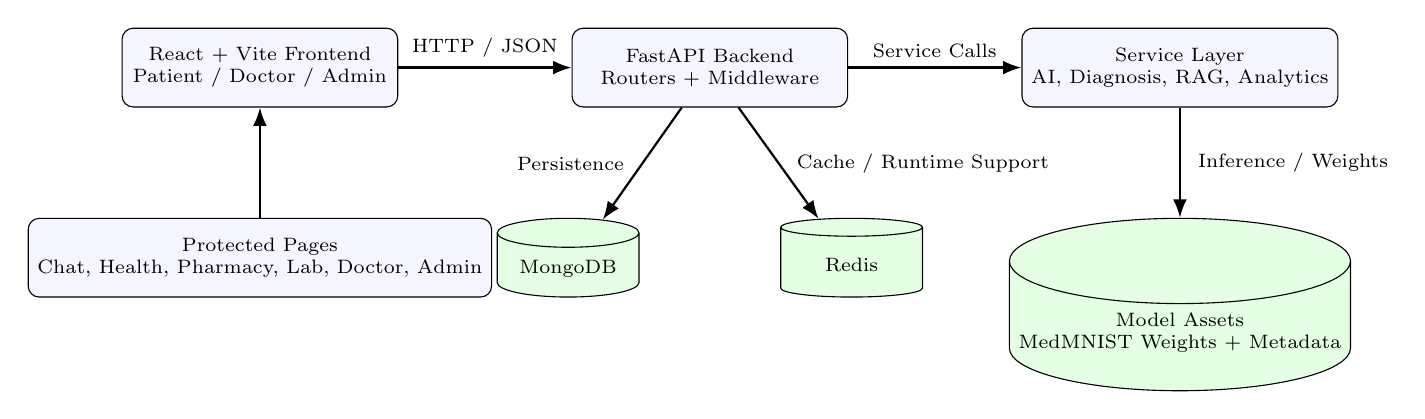
\begin{tikzpicture}[
    node distance=1.2cm and 2.2cm,
    box/.style={draw, rounded corners, align=center, minimum width=3.5cm, minimum height=1.0cm, fill=blue!4, font=\scriptsize},
    db/.style={draw, cylinder, shape border rotate=90, aspect=0.25, align=center, minimum height=1.0cm, minimum width=1.8cm, fill=green!10, font=\scriptsize},
    flow/.style={-Latex, thick}
]
\node[box] (ui) {React + Vite Frontend\\Patient / Doctor / Admin};
\node[box, right=of ui] (api) {FastAPI Backend\\Routers + Middleware};
\node[box, right=of api] (svc) {Service Layer\\AI, Diagnosis, RAG, Analytics};

\node[db, below=of api, xshift=-1.8cm, yshift=-0.2cm] (mongo) {MongoDB};
\node[db, below=of api, xshift=1.8cm, yshift=-0.2cm] (redis) {Redis};

\node[box, below=of ui, yshift=-0.2cm] (browser) {Protected Pages\\Chat, Health, Pharmacy, Lab, Doctor, Admin};
\node[db, below=of svc, yshift=-0.2cm] (models) {Model Assets\\MedMNIST Weights + Metadata};

\draw[flow] (ui) -- node[above, font=\scriptsize]{HTTP / JSON} (api);
\draw[flow] (api) -- node[above, font=\scriptsize]{Service Calls} (svc);
\draw[flow] (api) -- node[left, font=\scriptsize, xshift=-0.1cm]{Persistence} (mongo);
\draw[flow] (api) -- node[right, font=\scriptsize, xshift=0.1cm]{Cache / Runtime Support} (redis);
\draw[flow] (svc) -- node[right, font=\scriptsize, xshift=0.1cm]{Inference / Weights} (models);
\draw[flow] (browser) -- (ui);
\end{tikzpicture}%
}
\caption{High-level MedAI architecture. The frontend routes requests to the FastAPI backend, which orchestrates data access, AI services, diagnosis, and supporting workflows.}
\label{fig:architecture}
\end{figure*}

From an architectural perspective, the system is layered. The outermost layer is the user interface, which renders role-specific pages and navigates between them through React Router. The middle layer is the HTTP API, which validates input, authenticates requests, and routes operations to services. The service layer contains domain-specific logic such as AI generation, image preprocessing, RAG lookup, diagnosis orchestration, notification scheduling, and health analytics. The data layer consists of database access abstractions and persistent stores. This layered approach keeps concerns separated and makes the codebase easier to reason about.

The backend application is assembled in a single FastAPI entrypoint. At startup, it loads environment variables, connects to MongoDB and Redis, starts the reminder scheduler, and registers CORS and middleware. The API then includes routers for auth, chat, health, medicine, admin, doctor, lab tests, products, prescriptions, analysis, diagnosis, orders, and consultations. Each router exposes a focused subset of the product behavior. This is a practical way to maintain a monolithic backend while preserving internal structure.

The most important service-side abstraction for this paper is the medical image pipeline. Rather than letting routes call ML models directly, MedAI routes uploaded images through a service that performs the following steps: modality normalization, model selection, tensor preprocessing, inference, prediction formatting, disease context mapping, explanation generation, and response assembly. This service-based design makes it possible to integrate new datasets or modalities without changing endpoint behavior. The route simply calls the pipeline and returns the result.

The frontend mirrors this modularity. It uses authentication context, theme context, dashboard layout components, and lazy-loaded pages to keep the application responsive. Public routes are separated from protected patient, doctor, and admin routes. This prevents unauthorized access and also allows the UI to adapt to user role. The result is a complete healthcare application that does not collapse into a flat list of pages.

\section{Backend Implementation}
The backend is implemented in FastAPI, which is well suited to asynchronous request handling, typed schemas, and modular router composition. The main application defines a lifespan handler that connects to the database and Redis, then starts the medicine reminder scheduler in the background. This lifecycle approach ensures that startup and shutdown behavior are explicit. It also centralizes the handling of resource initialization and cleanup.

The application loads CORS middleware for local frontend origins and adds rate limiting and error handling middleware. This is important because the platform exposes AI endpoints that can be relatively expensive, and it also serves as a user-facing healthcare system in which stability matters. The rate limiter limits request volume per minute, and the error handler normalizes unexpected failures into a consistent response shape. These are not glamorous features, but they are necessary in production-facing systems.

Authentication is implemented with JWT tokens, bcrypt password hashing, and Google OAuth support. The auth routes cover registration, login, Google token exchange, profile access, logout, and profile updates. The architecture also supports user roles such as patient, doctor, and admin. This role information drives frontend route access and some backend behavior. Having role-aware authentication in place is a prerequisite for a medical platform because the information visible to a patient should differ from the information visible to a clinician or administrator.

The chat route uses the AI service to generate responses. It can persist chat sessions in MongoDB, retrieve conversation history, and optionally invoke RAG when requested. The upload flow accepts files, extracts text or descriptions where appropriate, and then routes the content through the AI response engine. This makes the chatbot more useful than a simple prompt box because it can handle documents as well as text.

The health routes manage logs and analytics. Users can create, update, retrieve, and delete health log entries. Those logs may contain vital signs, symptoms, notes, and mood information. A health analytics service then evaluates the collected data over time to produce trend summaries. This feature is valuable because it helps the product move beyond isolated interactions and into longitudinal care support.

The medical, pharmacy, lab, consultation, and order routes are part of the broader application ecosystem. Even if some of those modules are not the focus of the diagnosis paper, they matter because they define the downstream flow from AI guidance to actionable healthcare steps. After a diagnosis or recommendation, the user can book a consultation, view medications, track prescriptions, or browse tests. That is an important product-level advantage.

\section{Frontend Implementation}
The frontend uses React 18 with Vite for fast local development and efficient builds. It integrates React Router for navigation, Google OAuth for login, Tailwind CSS for styling, Framer Motion for motion, Lucide icons for UI glyphs, and Recharts for data visualization. The application structure uses lazy loading for most pages while eagerly loading the authentication flow. This is a sensible tradeoff because the login and registration screens are likely first-touch pages, while the more complex dashboard views can be deferred until needed.

Route structure is role-aware. Public pages include login, registration, and OAuth success. Protected patient routes include chatbot, health tracking, medicine reminders, pharmacy, lab tests, prescriptions, nearby doctors, profile, orders, consultations, medicine scanning, help, and about. Admin routes include dashboard, user management, role management, analytics, settings, and doctor creation. Doctor routes include dashboard, patient lists, consultations, appointments, prescriptions, profile, and settings. The router uses a shared protection component that checks authentication status and role access before rendering pages.

This design is important because a healthcare app often looks simple on the surface but becomes complex once different responsibilities are exposed. Patients need quick access to relevant actions. Doctors need worklists and summary views. Admins need configuration and analytics. The routing strategy used here is a clean way to handle that complexity without building separate applications.

The frontend also uses contextual providers for authentication and theme management. The auth provider likely stores token and user state, enabling the route guards to work consistently across page transitions. The theme provider supports visual consistency and could be extended to support user preferences. The dashboard layout component provides a shared frame for admin and doctor pages, while patient pages use direct routes with focused layouts. This division keeps the user experience coherent.

Table~\ref{tab:routes} maps the major frontend route groups to their primary responsibilities.

\begin{table}[H]
\centering
\caption{Representative Frontend Route Groups}
\label{tab:routes}
\begin{tabular}{p{0.32\linewidth} p{0.55\linewidth}}
\toprule
\textbf{Route Group} & \textbf{Representative Screens} \\
\midrule
Public & Login, Register, OAuth success \\
Patient & Chatbot, Health Tracking, Medicine Reminder, Pharmacy, Lab Tests \\
Doctor & Dashboard, Patients, Consultations, Appointments, Prescriptions \\
Admin & Dashboard, Users, Roles, Analytics, Settings, Create Doctor \\
\bottomrule
\end{tabular}
\end{table}

One notable implementation detail is the use of lazy loading for pages. This matters in a multi-module healthcare app because a large bundle can degrade usability. By deferring the loading of less frequently visited routes, the application keeps initial navigation faster. This is especially useful for users entering through login or chat, where responsiveness is important.

\begin{figure*}[t]
\centering
\fbox{\parbox{0.88\textwidth}{\centering
\vspace{12mm}
UI screenshot placeholder for MedAI dashboard/chat workflow.\\
Replace with the final exported interface figure before submission.
\vspace{12mm}
}}
\caption{MedAI user interface snapshot placeholder (replace with final captured UI figure in camera-ready version).}
\label{fig:website_ui}
\end{figure*}

\section{MedMNIST-Based Image Diagnosis}
The image diagnosis pipeline is the most technically specific part of the current branch. It reflects an explicit shift toward image-centric diagnosis with a controlled model selection strategy. Rather than using a generalized image prompt or treating every image as a free-form vision task, the platform loads a dedicated medical image classifier based on MedMNIST-compatible weights. The implementation uses EfficientNet-B0 as the backbone, which provides a reasonable balance between accuracy, parameter efficiency, and practical deployability.

Table~\ref{tab:modalities} summarizes the supported MedMNIST modalities and their key configuration fields.

\begin{table*}[t]
\centering
\caption{Supported MedMNIST Modalities and Model Metadata}
\label{tab:modalities}
\begin{tabular}{p{0.12\linewidth} p{0.18\linewidth} p{0.16\linewidth} p{0.22\linewidth} p{0.12\linewidth}}
\toprule
\textbf{Modality} & \textbf{Dataset Class} & \textbf{Task Name} & \textbf{Weight File} & \textbf{Type} \\
\midrule
Skin & DermaMNIST & dermamnist & efficientnet\_skin\_disease.pth & Single-label \\
Pathology & PathMNIST & pathmnist & efficientnet\_pathology\_disease.pth & Single-label \\
Chest & ChestMNIST & chestmnist & efficientnet\_chest\_disease.pth & Multi-label \\
OCT & OCTMNIST & octmnist & efficientnet\_oct\_disease.pth & Single-label \\
Pneumonia & PneumoniaMNIST & pneumoniamnist & efficientnet\_pneumonia\_disease.pth & Single-label \\
Retina & RetinaMNIST & retinamnist & efficientnet\_retina\_disease.pth & Single-label \\
Blood & BloodMNIST & bloodmnist & efficientnet\_blood\_disease.pth & Single-label \\
Tissue & TissueMNIST & tissuemnist & efficientnet\_tissue\_disease.pth & Single-label \\
Breast & BreastMNIST & breastmnist & efficientnet\_breast\_disease.pth & Single-label \\
Organ-A & OrganAMNIST & organamnist & efficientnet\_organa\_disease.pth & Single-label \\
Organ-C & OrganCMNIST & organcmnist & efficientnet\_organc\_disease.pth & Single-label \\
Organ-S & OrganSMNIST & organsmnist & efficientnet\_organs\_disease.pth & Single-label \\
\bottomrule
\end{tabular}
\end{table*}

MedMNIST is a useful choice for this type of work because it provides standardized 2D medical image subsets across several anatomical or diagnostic domains. The codebase supports a broad set of modalities, including skin, pathology, chest, OCT, pneumonia, retina, blood, tissue, breast, and organ-based subsets. Each modality is associated with metadata such as dataset class, task name, weight filename, and whether the problem is multi-label. This metadata is stored in a modality configuration map and used to determine both loading and normalization behavior.

The service that handles medical image inference first determines which modality to use. If the user requests a known modality, the system normalizes aliases into a supported key. If the requested modality is unspecified or marked as auto, the service prefers a skin model if available, otherwise it falls back to the first loaded model. This ensures that the pipeline can continue functioning even when not all modalities are present. In practical terms, that means a deployment can support a subset of the modalities without code changes.

The model loading logic scans for weight files in the backend weights directory. For each available file, the service extracts the model state dictionary and metadata, cleans any distributed-training prefixes, resolves class names, constructs an EfficientNet-based architecture, loads the weights, and sets the model to evaluation mode. If the checkpoint metadata includes a classifier shape, the class name list is adapted to match the number of output classes. This is a careful piece of engineering because it accommodates variation across training artifacts.

Preprocessing uses PIL and torchvision transforms. Images are resized to the expected input size, converted to RGB when necessary, turned into tensors, and normalized with ImageNet statistics. The implementation caches transforms by size so repeated inference does not reinstantiate them. Images are handled from raw bytes, which makes the service suitable for multipart uploads and also for internal pipelines that may pass image payloads in memory.

The prediction routine selects the active modality, preprocesses the image, runs the model under no-grad context, computes softmax probabilities for single-label tasks or sigmoid probabilities for multi-label tasks, and returns a structured result. The result includes the predicted disease, confidence, top predictions, threshold status, and modality metadata. The confidence threshold is used both to flag low-confidence outputs and to support disclaimers. For multi-label modalities such as ChestMNIST, thresholding is especially important because the label interpretation differs from single-class classification.

The pipeline does not stop at the prediction. It maps the disease output into a richer clinical context using a disease mapping utility. That mapping provides a doctor specialty, treatment hints, tests, and disease information. The system then generates an explanation, typically by prompting the AI service with the prediction, confidence, symptom input, specialist recommendation, suggested tests, and any retrieved knowledge snippets. This explanation is designed to be concise, compassionate, and clinically cautious.

The current architecture distinguishes between a basic visual description path and a clinical image path. The basic path uses the AI service to produce a non-diagnostic description of an image, and it is intended for general visual understanding rather than medical inference. The clinical path invokes the medical image pipeline and uses MedMNIST weights. This distinction is important because it prevents general vision tasks from being confused with diagnosis tasks. It is also a safer product design.

Figure~\ref{fig:flowchart} gives a simplified diagnosis flow chart that separates basic image description from clinical image inference.

\begin{figure*}[t]
\centering
\resizebox{0.85\textwidth}{!}{%
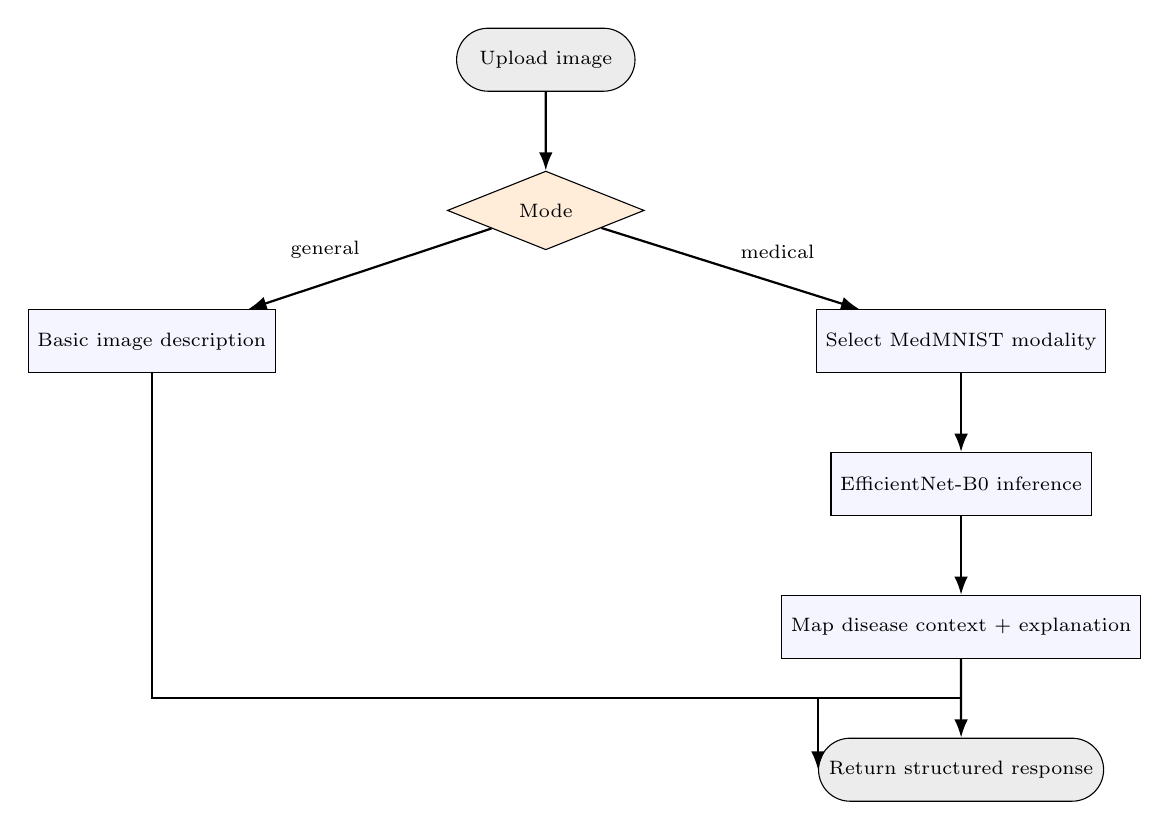
\begin{tikzpicture}[
    node distance=1.0cm and 1.8cm,
    startstop/.style={draw, rounded rectangle, minimum width=2.5cm, minimum height=0.8cm, fill=gray!15, align=center, font=\scriptsize},
    process/.style={draw, rectangle, minimum width=3.0cm, minimum height=0.8cm, fill=blue!4, align=center, font=\scriptsize},
    decision/.style={draw, diamond, aspect=2.0, minimum width=2.5cm, minimum height=1.0cm, fill=orange!15, align=center, font=\scriptsize},
    flow/.style={-Latex, thick}
]
\node[startstop] (start) {Upload image};
\node[decision, below=of start] (mode) {Mode};
\node[process, below left=of mode, xshift=-1.0cm] (basic) {Basic image description};
\node[process, below right=of mode, xshift=1.0cm] (clinical) {Select MedMNIST modality};
\node[process, below=of clinical] (infer) {EfficientNet-B0 inference};
\node[process, below=of infer] (context) {Map disease context + explanation};
\node[startstop, below=of context] (end) {Return structured response};

\draw[flow] (start) -- (mode);
\draw[flow] (mode) -- node[above left, font=\scriptsize]{general} (basic);
\draw[flow] (mode) -- node[above right, font=\scriptsize]{medical} (clinical);
\draw[flow] (clinical) -- (infer);
\draw[flow] (infer) -- (context);
\draw[flow] (context) -- (end);

% Connecting the basic description path to the end
\draw[flow] (basic.south) |- ($(end.north)!0.5!(context.south)$) -| (end.west);
\end{tikzpicture}%
}
\caption{Simplified image diagnosis flow. The system either produces a general visual description or follows the medical inference path with modality-specific model loading and response enrichment.}
\label{fig:flowchart}
\end{figure*}

\section{Diagnosis Orchestration and Response Design}
One of the strengths of MedAI is that diagnosis output is not returned as a bare classification label. The diagnosis orchestration service transforms the raw prediction into a structured response. This response includes the decision path, prediction details, doctor mapping, treatment context, suggested tests, disease information, an explanation string, module routes, and a disclaimer. This makes the endpoint useful to both frontend developers and end users.

The orchestration service enforces a clear decision path. If the modality is basic or general, the service does not claim to make a clinical prediction. Instead, it uses the AI service to describe the image and returns a general visual summary with a disclaimer that the mode is not a medical diagnosis. For image-based medical modalities, the service delegates to the image diagnosis service, then enriches the result with contextual information. This separation prevents accidental overreach and clarifies the intended behavior of each mode.

The response structure is especially well suited for user interface rendering. The frontend can present the predicted disease, confidence percentage, top predictions, and threshold indicator. It can also link directly into the doctor portal, prescription module, pharmacy, lab tests, reminders, and health tracking. In other words, the diagnosis result is already connected to the rest of the platform. This is a form of application-level interoperability that is often missing in standalone ML demos.

The explanation text is generated by the AI service using a prompt that describes the decision path, prediction, confidence, symptoms, recommended specialist, and test suggestions. If RAG is enabled, the pipeline tries to retrieve a small number of medically relevant knowledge snippets and fold them into the prompt. This means the language model is not operating from raw prediction alone. It is grounded in both structured disease context and optional retrieved documents. That is a better pattern for clinical explanation than a purely imaginative free-response prompt.

The system also considers failure scenarios. If the basic image mode cannot return a description, the service returns a helpful error message rather than silently failing. If the AI provider is not configured, the response instructs the operator to set the proper provider and key. If the medical image model is unavailable, the diagnosis endpoint can fail gracefully with a service-unavailable error. These are important behaviors because the platform should not obscure operational problems behind generic fallback text.

\section{AI Service Layer and Retrieval Augmentation}
The AI service is deliberately provider-agnostic. It can be configured to use Gemini, Hugging Face, OpenAI, or Ollama. This is useful for a healthcare application because provider availability, cost, privacy, and latency requirements can vary substantially across deployments. A local Ollama model may be attractive for offline or privacy-sensitive environments, while Gemini may be preferable for fast and cost-effective cloud inference. The code supports all of these as configuration options.

This design follows the broader trend in retrieval-augmented systems where the generation model is decoupled from the knowledge source and reasoning context \cite{rag}. It also aligns with modern application architectures in which the frontend, backend, and inference components are independently configurable \cite{fastapi,react,vite}.

The service initializes the selected provider, validates whether the corresponding API key is present, and then exposes common operations such as simple response generation, image description, and text extraction from images. If no valid API key is configured, the service returns a structured configuration message rather than throwing an unhelpful error. This makes misconfiguration easier to detect and remedy during deployment.

The general response prompt used by the AI service is concise and medically cautious. It instructs the model to act as a medical assistant, reply fast, keep answers organized, mention urgent warning signs when relevant, and avoid diagnosis or prescription behavior. This prompt discipline is necessary because a general-purpose language model can easily drift into overconfident medical advice if left unconstrained.

The retrieval-augmented generation component adds another layer of groundedness. When enabled, the AI service attempts to retrieve medical knowledge from a vector database or FAISS index. The retrieved content is then appended to the prompt context, allowing the model to produce explanations that are informed by more than the immediate user input. This is especially useful for medical support, where domain knowledge and caution are both important.

The platform also includes image text extraction functionality for document-style images such as lab reports, prescriptions, or discharge notes. In that workflow, the AI service can use Gemini vision to perform OCR-like extraction or a short description. This complements the medical image classifier by supporting documents and mixed input types in the chat module. It is a practical extension because many patients will upload paperwork rather than disease-specific images.

\section{Data, Models, and Modality Handling}
The model metadata layer is a central part of the image diagnosis system. Each modality is associated with a dataset class, task name, dataset identifier, weight filename, and label type. This metadata is not merely informational; it is used during model loading, modality normalization, and response construction. The system also defines common aliases so that terms like xray, lung, lungs, eye, organ-a, organ-c, and organ-s map to supported modalities. This improves usability because end users and frontend developers do not need to memorize internal keys.

Model asset management is a practical concern in systems like this. The codebase keeps weights under backend models and loads them dynamically if present. If a model file is missing, the service simply does not register that modality. This is a reasonable design because it allows the same codebase to run in partial-model or fully model-loaded deployments. It also makes local development easier, since a developer can test a subset of modalities without having every checkpoint available.

The code also keeps track of image size and backbone metadata. Although EfficientNet-B0 is the primary backbone in the current branch, the metadata system allows future flexibility. If a checkpoint records a different backbone or input size, the service can use those values to construct the model and preprocessing pipeline. This preserves compatibility with different training experiments and makes the runtime more robust.

A subtle but important design point is multi-label support. Some MedMNIST subsets, such as ChestMNIST, are multi-label rather than strictly single-class classification problems. The service therefore needs to adapt the post-processing logic depending on the modality. This is handled through metadata, with thresholds and prediction formatting adjusted accordingly. In other words, the system does not assume that every medical image task looks like a single-label classification problem.

\section{Security, Safety, and Reliability}
Healthcare applications must balance capability with caution. MedAI addresses this through several layers of safety and reliability mechanisms. First, authentication is mandatory for most user-facing operations. Second, role-based routing reduces exposure of administrative and clinical tools. Third, the diagnosis subsystem emits explicit disclaimers and distinguishes between preliminary assessment and final diagnosis. Fourth, the AI layer is prompted to avoid prescribing or overclaiming. These measures do not make the system clinically certified, but they do reduce the risk of misuse.

The platform also adds rate limiting and centralized error handling. In an application that exposes AI endpoints, rate limiting prevents accidental overuse and helps mitigate abuse. Error normalization is equally important because users should not see raw stack traces or inconsistent error payloads. The codebase routes these concerns through middleware so that the rest of the application remains focused on domain logic.

Operational reliability is strengthened by careful startup behavior. The backend checks the availability of the target port and exits gracefully if the service appears to already be running. This avoids noisy bind failures that can confuse developers. The Windows-specific handling of Uvicorn reload is also a practical detail because reloading a model-heavy FastAPI app can cause double initialization and break inference imports. The implementation therefore prefers an opt-in reload flag.

The image diagnosis path also handles missing inputs and malformed images. File type validation ensures that only image payloads reach the diagnosis logic. Empty uploads are rejected. Preprocessing failures raise explicit errors that can be surfaced to the client. These checks matter because image uploads are a frequent source of runtime issues in web applications.

Another reliability feature is service decomposition. The diagnosis route does not directly manipulate model tensors or AI prompts. Instead, it delegates to services that can be tested and improved independently. This reduces coupling and improves maintainability. If the AI provider changes, only the AI service needs adjustment. If a new modality is added, the model service and metadata configuration can be updated without rewriting the route layer.

\section{Implementation Patterns and Design Tradeoffs}
There are several notable implementation patterns in the MedAI codebase. One is the use of lazy loading in the frontend to optimize initial page performance. Another is the use of a shared AI service abstraction to hide the details of provider selection. A third is the decision to separate image diagnosis from general chat. This last choice is especially important and reflects an appropriate design tradeoff.

One tempting simplification in AI products is to push all reasoning through a single chatbot endpoint. That pattern is easy to build but hard to govern. It creates ambiguity about whether an answer came from a model, a retriever, a classifier, or a text prompt. MedAI avoids this problem by creating distinct pathways: chat for conversational assistance, analysis for general AI health guidance, and diagnosis for image-based medical prediction. This separation makes the product easier to validate and safer to explain.

Another tradeoff concerns model flexibility versus operational simplicity. The image diagnosis service supports multiple modalities and can load whichever weights are available. This adds complexity to the metadata layer, but it also makes the product more adaptable. A strictly single-modality system would be easier to reason about, but it would not match the broader MedMNIST integration goals of the project. The current approach is more ambitious and more useful in practice.

A further tradeoff is between rich explanations and concise output. The system attempts to keep explanations under a manageable length while still presenting enough detail to be actionable. This is a sensible compromise. In healthcare UX, overly long responses can overwhelm users, while overly short responses can feel cryptic. The prompt logic therefore asks the model to generate clear, concise, and compassionate explanations with specific sections.

\section{Experimental Setup and Results}
EfficientNet-B0 classifiers are trained using the standard MedMNIST v2 train/validation/test splits \cite{medmnistv2}. The canonical scripts are \texttt{train\_medmnist\_efficientnet.py} and \texttt{evaluate\_medmnist\_efficientnet.py}. The current repository state includes script-generated evaluation metrics for available checkpoints in \texttt{backend/models/weights/medmnist\_eval\_results.json}. Training/evaluation manifests and deterministic seed support are included in the scripts for reproducibility.

Table~\ref{tab:results} reports current script-aligned test-set metrics from the repository artifact (single-run values for available modalities/checkpoints). AUC is macro-averaged for multi-class tasks; Accuracy is top-1 for single-label tasks.

\begin{table*}[t]
\centering
\caption{Current script-generated EfficientNet-B0 test metrics from repository artifacts (\texttt{backend/models/weights/medmnist\_eval\_results.json})}
\label{tab:results}
\begin{tabular}{p{0.16\linewidth} p{0.14\linewidth} p{0.12\linewidth} p{0.12\linewidth} p{0.38\linewidth}}
\toprule
\textbf{Modality} & \textbf{Task} & \textbf{AUC} & \textbf{ACC} & \textbf{Note} \\
\midrule
DermaMNIST & Multi-class (7) & 0.5049 & 0.1062 & Script output from current available checkpoint \\
PathMNIST  & Multi-class (9) & 0.5214 & 0.0586 & Script output from current available checkpoint \\
OCTMNIST   & Multi-class (4) & 0.4179 & 0.2500 & Script output from current available checkpoint \\
PneumoniaMNIST & Binary (2) & 0.5700 & 0.3750 & Script output from current available checkpoint \\
RetinaMNIST & Ordinal (5) & 0.5152 & 0.4350 & Script output from current available checkpoint \\
BreastMNIST & Binary (2) & 0.4337 & 0.7308 & Script output from current available checkpoint \\
\bottomrule
\end{tabular}
\end{table*}

These values represent the current artifact state in the repository and should be interpreted as implementation-validation results, not final benchmark-optimized scores. Full modality coverage depends on available checkpoint files in \texttt{backend/models/weights}. The same script and schema support additional modalities when their weights are present.

\section{Evaluation Considerations}
The repository includes a formal evaluation script that runs each modality checkpoint against the MedMNIST v2 held-out test split and reports accuracy, macro F1, and macro AUC. Table~\ref{tab:results} in the previous section presents the primary results for six modalities. Several additional evaluation axes are worth noting for a complete picture of the platform.

The first is functional correctness: do routes authenticate properly, persist records, and return expected payloads? The second is model integration correctness: do modality weights load successfully, and does the image diagnosis service produce structured outputs? The third is UI responsiveness: do lazy-loaded routes and layout components keep the interface usable on common devices? The fourth is operational robustness: does the backend start reliably, handle missing services, and respond gracefully to misconfiguration?

For the diagnosis subsystem, a useful evaluation protocol includes modality-specific tests. Each supported MedMNIST checkpoint should be validated for successful load, preprocessing compatibility, output shape, threshold behavior, and result formatting. In addition, the API response should be verified for edge cases such as missing image uploads, unsupported file types, missing model weights, and auto modality fallback. These checks ensure that the pipeline behaves as intended across supported use cases.

From a product perspective, user feedback would likely focus on trust and clarity. Users need to know whether the system is offering a general description, a preliminary assessment, or a supported clinical image prediction. The system’s disclaimers and route separation help with that, but interface design still matters. Future evaluation should therefore include usability studies centered on whether users understand the limits of each mode.

\section{Limitations}
The system is powerful, but it has clear limitations. First, it is still an AI-assisted platform rather than a clinically certified diagnostic product. Its outputs should not be used as a substitute for professional medical advice. Second, the quality of image diagnosis depends on the availability and quality of the trained MedMNIST weights. Third, modality support is bounded by the datasets and checkpoints that have been configured. Fourth, AI explanations depend on the selected provider and the quality of the prompt or retrieved knowledge.

Another limitation is that the repository mixes several concerns in one codebase. This is practical for a project of this size, but larger production deployments might eventually split services into separate repositories or deploy them independently. For example, the model training script, inference service, and product UI could be separated for organizational clarity. At the current scale, however, the monorepo structure is reasonable.

The current implementation also depends on external services such as MongoDB, Redis, and an AI provider. If these services are unavailable, some features degrade or fail. The code does include fallback behavior, but operational quality still depends on proper environment setup. This is normal for an integrated healthcare platform, but it is important to acknowledge.

\section{Future Work}
Several extensions would make MedAI stronger. The first would be a formal evaluation suite for the medical image diagnosis pipeline, including unit tests for modality normalization, integration tests for model loading, and end-to-end tests for the diagnosis route. The second would be a richer explanation layer that distinguishes between evidence-backed and heuristic suggestions. The third would be a more explicit model registry or versioning system so that multiple checkpoint versions can be tracked over time.

A fourth extension would be broader frontend feedback around confidence and modality selection. The UI could allow users to see why a particular modality was chosen, what alternative modes are available, and how the confidence threshold influences the displayed recommendation. A fifth extension would be stronger clinical workflow integration, such as handoff to telemedicine, follow-up tasks, or secure export of summary reports.

Another promising direction is dataset and modality expansion. The current project already spans a wide range of MedMNIST subsets, but future versions could add support for more task-specific model families or more robust multi-label handling. A more advanced version might also include uncertainty calibration, explainability visualizations such as saliency maps, or a clinician review mode where predictions are logged and reviewed rather than immediately shown to patients.

Finally, the chat and diagnosis subsystems could be more tightly integrated in a safe way. For example, a patient could upload an image, receive a structured preliminary assessment, and then ask follow-up questions in chat that are explicitly grounded in that assessment and the retrieved medical references. That would preserve the distinction between diagnosis and chat while improving continuity.

\section{Conclusion}
MedAI demonstrates how a modern web application can combine healthcare workflows, conversational AI, medical image classification, and role-based user experience into a single coherent platform. The project is not simply a chat app with an image upload field. It is a layered system that treats diagnosis, support, scheduling, tracking, and administration as complementary components of a broader patient care experience. The current MedMNIST integration is especially noteworthy because it reorients diagnosis around actual image inference with EfficientNet-B0 models, modality-aware handling, and structured downstream guidance.

From a software engineering perspective, the project shows careful separation of concerns. The backend centralizes resource management and service orchestration. The frontend uses lazy-loaded, role-aware routing. The AI layer abstracts over multiple providers and RAG retrieval. The image diagnosis service manages model loading, modality normalization, and preprocessing. Together, these choices create a system that is practical, extensible, and easier to operate than an ad hoc prototype.

From an applied AI perspective, MedAI illustrates an important principle: model output alone is not enough. Users need context, explanation, thresholds, and next steps. The value of the system comes from connecting medical image classification to real application behavior such as specialist mapping, test suggestions, prescriptions, pharmacy support, and reminders. That connection is what turns a model demo into a usable healthcare product.

Table~\ref{tab:api} summarizes several of the key backend API areas discussed throughout the paper.

\begin{table}[H]
\centering
\caption{Representative Backend API Surfaces}
\label{tab:api}
\begin{tabular}{p{0.34\linewidth} p{0.48\linewidth}}
\toprule
\textbf{Endpoint Area} & \textbf{Purpose} \\
\midrule
Auth & Login, registration, Google OAuth, profile management \\
Chat & General AI chat, session management, file uploads \\
Health & Logs, analytics, and health trend tracking \\
Diagnosis & MedMNIST image inference and structured clinical context \\
Analysis & AI-based general health analysis and symptoms support \\
\bottomrule
\end{tabular}
\end{table}

\begin{thebibliography}{99}

\bibitem{fastapi}
S. Ramírez, ``FastAPI Documentation,'' accessed 2026. Available: \url{https://fastapi.tiangolo.com/}

\bibitem{react}
Meta, ``React Documentation,'' accessed 2026. Available: \url{https://react.dev/}

\bibitem{vite}
Vite, ``Vite Documentation,'' accessed 2026. Available: \url{https://vite.dev/}

\bibitem{medmnistv2}
J. Yang, R. Shi, D. Wei, Z. Liu, L. Zhao, B. Ke, H. Pfister, and B. Ni, ``MedMNIST v2: A Large-Scale Lightweight Benchmark for 2D and 3D Biomedical Image Classification,'' \emph{Scientific Data}, vol. 10, no. 1, p. 41, 2023.

\bibitem{efficientnet}
M. Tan and Q. Le, ``EfficientNet: Rethinking Model Scaling for Convolutional Neural Networks,'' in \emph{ICML}, 2019.

\bibitem{esteva}
A. Esteva et al., ``Dermatologist-level classification of skin cancer with deep neural networks,'' \emph{Nature}, vol. 542, pp. 115--118, 2017.

\bibitem{chexnet}
P. Rajpurkar et al., ``CheXNet: Radiologist-Level Pneumonia Detection on Chest X-Rays with Deep Learning,'' arXiv:1711.05225, 2017.

\bibitem{topol}
E. J. Topol, ``High-performance medicine: the convergence of human and artificial intelligence,'' \emph{Nature Medicine}, vol. 25, pp. 44--56, 2019.

\bibitem{pytorch}
A. Paszke et al., ``PyTorch: An Imperative Style, High-Performance Deep Learning Library,'' in \emph{NeurIPS}, 2019.

\bibitem{mongodb}
MongoDB, Inc., ``MongoDB Manual,'' accessed 2026. Available: \url{https://www.mongodb.com/docs/}

\bibitem{redis}
Redis Ltd., ``Redis Documentation,'' accessed 2026. Available: \url{https://redis.io/docs/}

\bibitem{rag}
P. Lewis et al., ``Retrieval-Augmented Generation for Knowledge-Intensive NLP Tasks,'' in \emph{NeurIPS}, 2020.

\end{thebibliography}

\end{document}
